%% ****** Start of file apstemplate.tex ****** %
%%
%%
%%   This file is part of the APS files in the REVTeX 4.2 distribution.
%%   Version 4.2a of REVTeX, January, 2015
%%
%%
%%   Copyright (c) 2015 The American Physical Society.
%%
%%   See the REVTeX 4 README file for restrictions and more information.
%%
%
% This is a template for producing manuscripts for use with REVTEX 4.2
% Copy this file to another name and then work on that file.
% That way, you always have this original template file to use.
%
% Group addresses by affiliation; use superscriptaddress for long
% author lists, or if there are many overlapping affiliations.
% For Phys. Rev. appearance, change preprint to twocolumn.
% Choose pra, prb, prc, prd, pre, prl, prstab, prstper, or rmp for journal
%  Add 'draft' option to mark overfull boxes with black boxes
%  Add 'showkeys' option to make keywords appear
%\documentclass[aps,prl,preprint,groupedaddress]{revtex4-2}
\documentclass[aps,prl,twocolumn,groupedaddress]{revtex4-2}
%\documentclass[aps,prl,preprint,superscriptaddress]{revtex4-2}
%\documentclass[aps,prl,reprint,groupedaddress]{revtex4-2}

% You should use BibTeX and apsrev.bst for references
% Choosing a journal automatically selects the correct APS
% BibTeX style file (bst file), so only uncomment the line
% below if necessary.
%\bibliographystyle{apsrev4-2}

\usepackage{graphicx}
\usepackage{subcaption}
\usepackage{caption}
\usepackage[font={small,it}]{caption}

\usepackage{epstopdf}
%\usepackage{amsmath}% http://ctan.org/pkg/amsmath
%\usepackage{amsthm}
%\usepackage{amsfonts}
%\usepackage{subfigure}
%\usepackage{hhline}
%\usepackage[miktex]{gnuplottex}
%\usepackage{xcolor}
\usepackage{amssymb}
\usepackage{amsmath}
\usepackage{color}
\usepackage{hyperref}
%\usepackage[percent]{overpic}
\usepackage{tikz}
\usepackage{mathrsfs}
\usepackage{wasysym}
\usepackage{tikz-cd}
%\usepackage{stix} %\fisheye
\usepackage{stackengine,scalerel}

% so sections, subsections, etc. become numerated.
\setcounter{secnumdepth}{3}

% Comandos proprios
\DeclareMathOperator*{\argmax}{arg\,max}
\DeclareMathOperator*{\argmin}{arg\,min}
\newcommand{\avrg}[1]{\left\langle #1 \right\rangle}
\newcommand{\nelta}{\bar{\delta}}
\newcommand{\bra}[1]{\left\langle #1\right|}
\newcommand{\ket}[1]{\left| #1 \right\rangle}
\newcommand{\sbra}[1]{\langle #1|}
\newcommand{\sket}[1]{| #1 \rangle}
\newcommand{\bek}[3]{\left\langle #1 \right| #2 \left| #3 \right\rangle}
\newcommand{\sbek}[3]{\langle #1 | #2 | #3 \rangle}
\newcommand{\braket}[2]{\left\langle #1 \middle| #2 \right\rangle}
\newcommand{\ketbra}[2]{\left| #1 \middle\rangle \middle\langle #2  \right|}
\newcommand{\sbraket}[2]{\langle #1 | #2 \rangle}
\newcommand{\sketbra}[2]{| #1 \rangle  \langle #2 |}
\newcommand{\norm}[1]{\left\lVert#1\right\rVert}
\newcommand{\snorm}[1]{\lVert#1\rVert}
\newcommand{\bvec}[1]{\boldsymbol{\mathsf{#1}}}
\newcommand{\bcov}[1]{\boldsymbol{#1}}
\newcommand{\bdua}[1]{\boldsymbol{\check{#1}}}
%\newcommand{\bdov}[1]{\boldsymbol{\breve{#1}}}
\newcommand{\bdov}[1]{\breve{#1}}
%\newcommand{\bten}[1]{\boldsymbol{\mathfrak{#1}}}
\newcommand{\bten}[1]{\boldsymbol{\mathfrak{#1}}}
\newcommand{\forany}{\tilde{\forall}}
\newcommand{\qed}{$\overset{\circ}{.}\;$}

\newcommand\bigeye{\ensurestackMath{\stackinset{c}{}{c}{-.3pt}%
  {\bullet}{\scriptstyle\bigcirc}}}
\newcommand\eye{\scalerel*{\bigeye}{x}}
%\newcommand*{\fisheye}{%
%    \mathbin{%
%        \ooalign{$\circledcirc$\cr\hidewidth$\bullet$\hidewidth}%
%    }%
%}
\renewcommand{\appendixname}{Apéndice} % Change "Appendix" to "Apéndice"

\begin{document}

% Use the \preprint command to place your local institutional report
% number in the upper righthand corner of the title page in preprint mode.
% Multiple \preprint commands are allowed.
% Use the 'preprintnumbers' class option to override journal defaults
% to display numbers if necessary
%\preprint{}

%Title of paper
\title{
Estudio del modelo de Hodgkin y Huxley
}

% repeat the \author .. \affiliation  etc. as needed
% \email, \thanks, \homepage, \altaffiliation all apply to the current
% author. Explanatory text should go in the []'s, actual e-mail
% address or url should go in the {}'s for \email and \homepage.
% Please use the appropriate macro foreach each type of information

% \affiliation command applies to all authors since the last
% \affiliation command. The \affiliation command should follow the
% other information
% \affiliation can be followed by \email, \homepage, \thanks as well.
\author{Luis Miguel Vargas Calderon}
\email[]{miguel.vargas@unc.edu.ar}
%\homepage[]{Your web page}
%\thanks{}
%\altaffiliation{}
%\affiliation{}
\affiliation{Facultad de Matem\'atica, Astronom\'ia, F\'isica y Computaci\'on, Universidad Nacional de C\'ordoba, Ciudad Universitaria, 5000 C\'ordoba, Argentina}

\author{Daniela Ruiz}
\email[]{danniela.vr31@gmail.com}
\affiliation{Facultad de Matem\'atica, Astronom\'ia, F\'isica y Computaci\'on, Universidad Nacional de C\'ordoba, Ciudad Universitaria, 5000 C\'ordoba, Argentina}

%Collaboration name if desired (requires use of superscriptaddress
%option in \documentclass). \noaffiliation is required (may also be
%used with the \author command).
%\collaboration can be followed by \email, \homepage, \thanks as well.
%\collaboration{Juan Perez}
%\noaffiliation

\date{\today}

\begin{abstract}
El objetivo de este trabajo es estudiar el comportamiento del modelo de Hodgkin-Huxley, utilizando métodos de integración numérica.
\end{abstract}

% insert suggested keywords - APS authors don't need to do this
%\keywords{}

%\maketitle must follow title, authors, abstract, and keywords
\maketitle

\section{Introducción}

El modelo de Hodgkin y Huxley describe cómo se inician y transmiten los potenciales de acción en las neuronas.

Consiste en un conjunto de cuatro ecuaciones diferenciales ordinarias acopladas no lineales, que aproximan las características eléctricas de células excitables como las neuronas.~\cite{HodgkinyHuxleyWikipedia}.

\section{Teoría}

Las siguientes ecuaciones diferenciales
detalladas en ~\cite{HodgkinyHuxleyWikipedia} 
son las que modelan el comportamiento de la neurona en función del cambio de la diferencia del potencial de la membrana que proteje a la neurona. Es decir en función de la razon de cambio del potencial $v$ entre el interior y el exterior de la membrana a lo largo del tiempo y a su vez en función de las probabilidades de activación o inactivación de ciertos canales internos de la membrana  que dependen del cambio de potencial antes mencionado, cuando la membrana es ejercitada con impulsos de iones.

\begin{eqnarray*}
\dot{n}&=&\alpha_n(v)(1-n)-\beta_n(v) n\\
\dot{m}&=&\alpha_m(v)(1-m)-\beta_m(v) m\\
\dot{h}&=&\alpha_h(v)(1-h)-\beta_h(v) h\\
\dot{v}&=&c^{-1}(i-\bar{g}_{\mathrm{Na}}m^3h(v-v_{\mathrm{Na}})-\bar{g}_{\mathrm{K}}n^4(v-v_{\mathrm{K}})-g_{l}(v-v_{l}))
\end{eqnarray*}
Acá $\dot{n}$, $\dot{m}$ y $\dot{h}$
representan la razon de cambio de las fracciones de canales de sodio  $Na$ abiertas, la razon de cambio de las fracciones de canales de potasio $K$ abiertas y la razon de cambio de las fracciones de canales de sodio $Na$ inactivos, respectivamente permitiendo el paso de iones a traves de la membrana. $\dot{v}$ representa la diferencia del potencial de la membrana.
Las tres primeras ecuaciones dependen del potencial. Cuando el potencial sufre un cambio, debido a una inyección o interrupción de iones, las fracciones de canales de cada tipo suben o bajan abriendo o cerrando los canales.


Utilizando el método de integración de Runge-Kutta de 4to orden  sobre el sistema de ecuaciones se logra aproximar las trayectorias de dichas variables.


Para estudiar el comportamiento de la neurona se definieron varias funciones que modelan el impulso de corriente de iones
denominadas como $i$, $i2$, etc.
La función de integración toma como parametros las ecuaciones diferenciales que a su vez en cada expermiento estan parametrizadas por cada una de las funciones de corrientes.
 

\section{Resultados}
Se realizaron 5 experimentos.

Experimento 1: \textbf{Valores de equilibrio}. Se utilizo una función de corriente que devuelve la constante 0. El objetivo es analizar como es el estado estacionario de la neurona cuando no recibe corriente.
Para integrar numericamente el sistema, se parametrizo con los siguientes valores iniciales:

\begin{eqnarray*}
{v}&=&0.0:&potencial de la membrana\\
{nt}&=&0.0:&probabilidad de activacion de K (potasio)\\
{mt}&=&0.0:&probabilidad de activacion de Na (sodio)\\
{ht}&=&0.0:probabilidad de inactivacion Na (sodio)\\
&
\end{eqnarray*}

Cuando inicia el modelado en los primeros [ms] El potencial de la membrana sufre un pico pero luego se estabiliza en 0. fig.~\ref{fig1}.

\begin{figure}[h!]
\centering
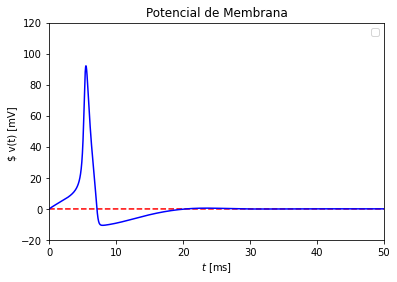
\includegraphics[scale=.4]{figs/potencial_de_membrana.png}
%\vspace{-0.25cm}
\caption{Potencial de membrana con función de corriente constante 0. \label{fig1}}
\end{figure}


Como resultado de la razon de cambio del potencial anterior en los primeros [ms] las fracciones de canales activos de sodio $n(t)$ se estabilizan en aproximadamente 0.6. La fracción de canales de Potasio $m(t)$ se estabilizan en aproximadamente 0.3 y la fracción de canales inactivos de sodio $h(t)$ se estabilizan aproximadamente por encima de 0. Esto se da para ${t \to \infty}$. fig.~\ref{fig2}. Estos son valores de equilibrio que seran utilizados como valores iniciales en los siguientes experimentos.


\begin{figure}[h!]
\centering
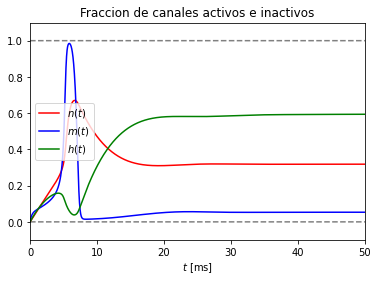
\includegraphics[scale=.4]{figs/fraccion_de_canales_activos_e_inactivos}
%\vspace{-0.25cm}
\caption{Fracción de canales activos e inactivos. \label{fig2}}
\end{figure}


Experimento 2: \textbf{Estímulo débil y estímulo fuerte}. Se utilizo la siguiente función de corriente $i2$.
$$
i2(t) = \left\{
\begin{array}{ll}
10 \mu A/cm^2, & t\in [2ms,2.5ms] \\
30 \mu A/cm^2, & t\in [10ms,10.5ms] \\
0 \mu A/cm^2, & c.c. \\
\end{array}
\right.
$$
En fig.~\ref{fig3}. se observa  que la cantidad de amperes inyectados en el periodo de tiempo [2ms,2.5ms]  no es suficiente como para activar el potencial de membrana. Sin embargo en el periodo de tiempo [10ms,12.5ms], el potencial de membrana alcanza un pico que  dispara la activación de las fracciones de canales activos e inactivos.  fig.~\ref{fig4}. 

\begin{figure}[h!]
\centering
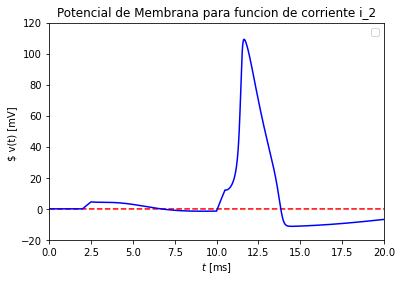
\includegraphics[scale=.4]{figs/potencial_membrana_i_2.png}
%\vspace{-0.25cm}
\caption{Potencial de membrana función i2. \label{fig3}}
\end{figure}

En concreto se observa que la Fracción de $nt$ y $mt$ sube a valores altos entre [0.8, 1] y baja a cerca de  0 para $h(t)$ en el periodo de tiempo [10ms,12.5ms], 
fig.~\ref{fig4}. lo cual indica que en ese periodo de tiempo la carga de iones puede pasar por la membrana.
Luego del disparo, las fracciones vuelven a valores de equilibrio.
Observar que este modelo inicia en los valores de equilibrio obtenidos en el experimento 1).\newline


\begin{figure}[h!]
\centering
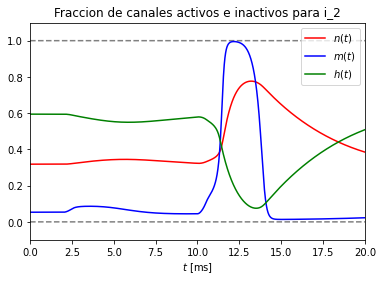
\includegraphics[scale=.4]{figs/fraccion_de_canales_activos_e_inactivos_para_i_2.png}
%\vspace{-0.25cm}
\caption{Fracción de canales activos e inactivos i2. \label{fig4}}
\end{figure}

Experimento 3: \textbf{Ráfaga}. Se utilizo la siguiente función de corriente $i3$ para modelar una rafaga de carga de iones.
$$
i3(t) = \left\{
\begin{array}{ll}
10 \mu A/cm^2, & t\in [5ms,\infty ms) \\
0 \mu A/cm^2, & c.c. \\
\end{array}
\right.
$$

Luego de 5[ms] se envía constantemente 10$uA$
El potencial se activa siempre a partir de ese tiempo y hasta el infinito.
Luego de unos [ms] vuelve a estado refractario y luego vuelve a disparar en un ciclo infinito. fig.~\ref{fig5}.



\begin{figure}[h!]
\centering
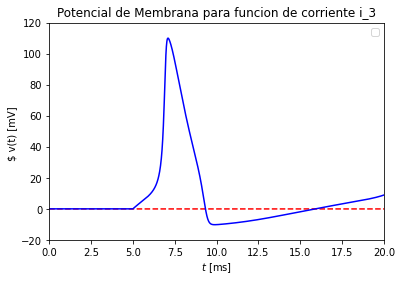
\includegraphics[scale=.4]{figs/potencial_membrana_i_3.png}
%\vspace{-0.25cm}
\caption{Potencial de membrana función i3. \label{fig5}}
\end{figure}

Al igual que en el experimento 2 se observa que las fracciones de canales activos e inactivos inician a partir de los valores de equilibrio.fig.~\ref{fig6}.
Ahora en un ciclo infinito $n(t)$ y $m(t)$ suben a valores altos entre
[0.8, 1] y luego vuelven a bajar a sus respectivos (aprox. 0.3), (aprox. 0.0), valores de equilibrio, 
y $h(t)$ baja a cerca de 0   luego vuelve a subir a su valor de equilibrio. (aprox. 0.6).



\begin{figure}[h!]
\centering
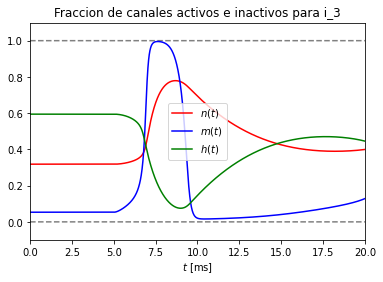
\includegraphics[scale=.4]{figs/fraccion_de_canales_activos_e_inactivos_para_i_3.png}
%\vspace{-0.25cm}
\caption{Fracción de canales activos e inactivos i3. \label{fig6}}
\end{figure}


Experimento 4: \textbf{Período refractario}. Se utilizo la siguiente función de corriente $i4$ para analizar un período refractario.
$$
i4(t) = \left\{
\begin{array}{ll}
10 \mu A/cm^2, & t\in [10ms\, k,10 ms\, k + 2ms], k > 0\\
0 \mu A/cm^2, & c.c. \\
\end{array}
\right.
$$

En fig.~\ref{fig7}. se observa  que 
XXXXXXXXXXXX.  

XXXXXXXXXXXX
XXXXXXXXXXXX
XXXXXXXXXXXX
XXXXXXXXXXXX
XXXXXXXXXXXX
XXXXXXXXXXXX
XXXXXXXXXXXX
XXXXXXXXXXXX
XXXXXXXXXXXX
XXXXXXXXXXXX


\begin{figure}[h!]
\centering
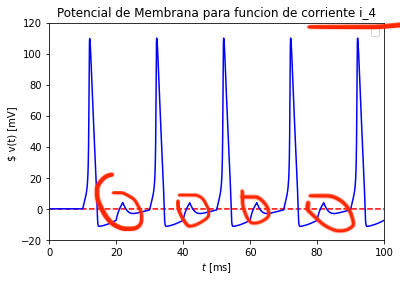
\includegraphics[scale=.4]{figs/potencial_membrana_i_4.png}
%\vspace{-0.25cm}
\caption{Potencial de membrana función i4.\label{fig7}}
\end{figure}
\begin{figure}[h!]

fig.~\ref{fig8}.
XXXXXXXXXXXX
XXXXXXXXXXXX
XXXXXXXXXXXX
XXXXXXXXXXXX
XXXXXXXXXXXX
XXXXXXXXXXXX
XXXXXXXXXXXX
XXXXXXXXXXXX


\centering
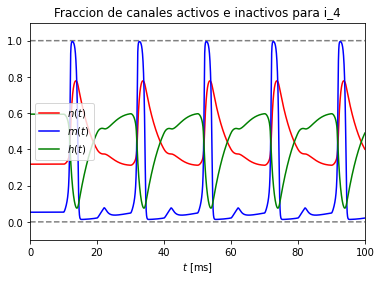
\includegraphics[scale=.4]{figs/fraccion_de_canales_activos_e_inactivos_para_i_4.png}
%\vspace{-0.25cm}
\caption{Fracción de canales activos e inactivos i4. \label{fig8}}
\end{figure}



Experimento 5: \textbf{Exitaciones espontáneas en respuesta al ruido}. Se utilizo la siguiente función de corriente $i5(t)\sim i_0 N(0,1)$ (i.e. $i_0$ por un valor aleatorio obtenido de una distribución normal de media 0 y varianza 1) para cada valor de $t$ en el que sea evaluada.

La corriente en este experimento se modela como un flujo de impulsos aleatorios.

En fig.~\ref{fig9}.


XXXXXXXXXXXX
XXXXXXXXXXXX
XXXXXXXXXXXX
XXXXXXXXXXXX
XXXXXXXXXXXX
XXXXXXXXXXXX
XXXXXXXXXXXX

XXXXXXXX  fig.~\ref{fig10}.
Observar que este modelo inicia en los valores de equilibrio obtenidos en el experimento 1).




\begin{figure}[h!]
\centering
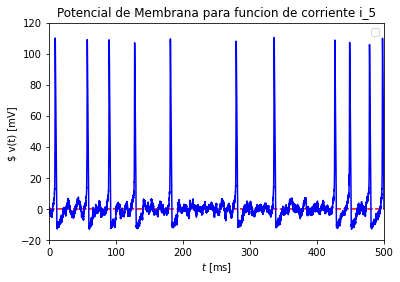
\includegraphics[scale=.4]{figs/potencial_membrana_i_5.png}
%\vspace{-0.25cm}
\caption{Potencial de membrana función i5. \label{fig9}}
\end{figure}



XXXXXXXXXXXX
XXXXXXXXXXXX
XXXXXXXXXXXX
XXXXXXXXXXXX
XXXXXXXXXXXX
XXXXXXXXXXXX
XXXXXXXXXXXX
XXXXXXXXXXXX



\begin{figure}[h!]
\centering
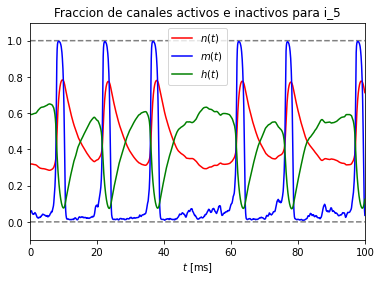
\includegraphics[scale=.4]{figs/fraccion_de_canales_activos_e_inactivos_para_i_5.png}
%\vspace{-0.25cm}
\caption{Fracción de canales activos e inactivos i5. \label{fig10}}
\end{figure}



XXXXXXXXXXXX
XXXXXXXXXXXX
XXXXXXXXXXXX
XXXXXXXXXXXX
XXXXXXXXXXXX
XXXXXXXXXXXX
XXXXXXXXXXXX
XXXXXXXXXXXX



\section{Discusión}

La comparación de ................................................................
...............................................................
.. bla bla bla ................................................................
...............................................................
.. bla bla bla

\section{Conclusiones}

Consideramos que estudiar el modelo de Hodgkin y Huxley es muy propicio para poner en practica los conocimientos adqueridos en cuanto a resolucion de sistema de ecuaciones diferenciales. Utilizar herramientas de integracion numerica como RK4 implementado en python es tambien un buen inicio para profundizar el conocimiento en redes neuronales.


% If in two-column mode, this environment will change to single-column
% format so that long equations can be displayed. Use
% sparingly.
%\begin{widetext}
% put long equation here
%\end{widetext}

% figures should be put into the text as floats.
% Use the graphics or graphicx packages (distributed with LaTeX2e)
% and the \includegraphics macro defined in those packages.
% See the LaTeX Graphics Companion by Michel Goosens, Sebastian Rahtz,
% and Frank Mittelbach for instance.
%
% Here is an example of the general form of a figure:
% Fill in the caption in the braces of the \caption{} command. Put the label
% that you will use with \ref{} command in the braces of the \label{} command.
% Use the figure* environment if the figure should span across the
% entire page. There is no need to do explicit centering.

% \begin{figure}
% \includegraphics{}%
% \caption{\label{}}
% \end{figure}

% Surround figure environment with turnpage environment for landscape
% figure
% \begin{turnpage}
% \begin{figure}
% \includegraphics{}%
% \caption{\label{}}
% \end{figure}
% \end{turnpage}

% tables should appear as floats within the text
%
% Here is an example of the general form of a table:
% Fill in the caption in the braces of the \caption{} command. Put the label
% that you will use with \ref{} command in the braces of the \label{} command.
% Insert the column specifiers (l, r, c, d, etc.) in the empty braces of the
% \begin{tabular}{} command.
% The ruledtabular enviroment adds doubled rules to table and sets a
% reasonable default table settings.
% Use the table* environment to get a full-width table in two-column
% Add \usepackage{longtable} and the longtable (or longtable*}
% environment for nicely formatted long tables. Or use the the [H]
% placement option to break a long table (with less control than 
% in longtable).
% \begin{table}%[H] add [H] placement to break table across pages
% \caption{\label{}}
% \begin{ruledtabular}
% \begin{tabular}{}
% Lines of table here ending with \\
% \end{tabular}
% \end{ruledtabular}
% \end{table}

% Surround table environment with turnpage environment for landscape
% table
% \begin{turnpage}
% \begin{table}
% \caption{\label{}}
% \begin{ruledtabular}
% \begin{tabular}{}
% \end{tabular}
% \end{ruledtabular}
% \end{table}
% \end{turnpage}

%\section{Aknowledgments}
\section{Agradecimientos}

\begin{acknowledgments}
a FaMAF, siempre FaMAF y a la educación publica.
\end{acknowledgments}
% Create the reference section using BibTeX:
\bibliography{ref}

% Specify following sections are appendices. Use \appendix* if there
% only one appendix.

\onecolumngrid

\appendix


\end{document}
%
% ****** End of file apstemplate.tex ******


